\section{ローズ・ピアノの物理モデル}

本章ではローズ・ピアノ振動体を簡略化した物理モデルを検討する.簡易モデルに使用するシステムモデルを図\ref{fig:簡易モデル}に示す.

\begin{figure}
    \centering
    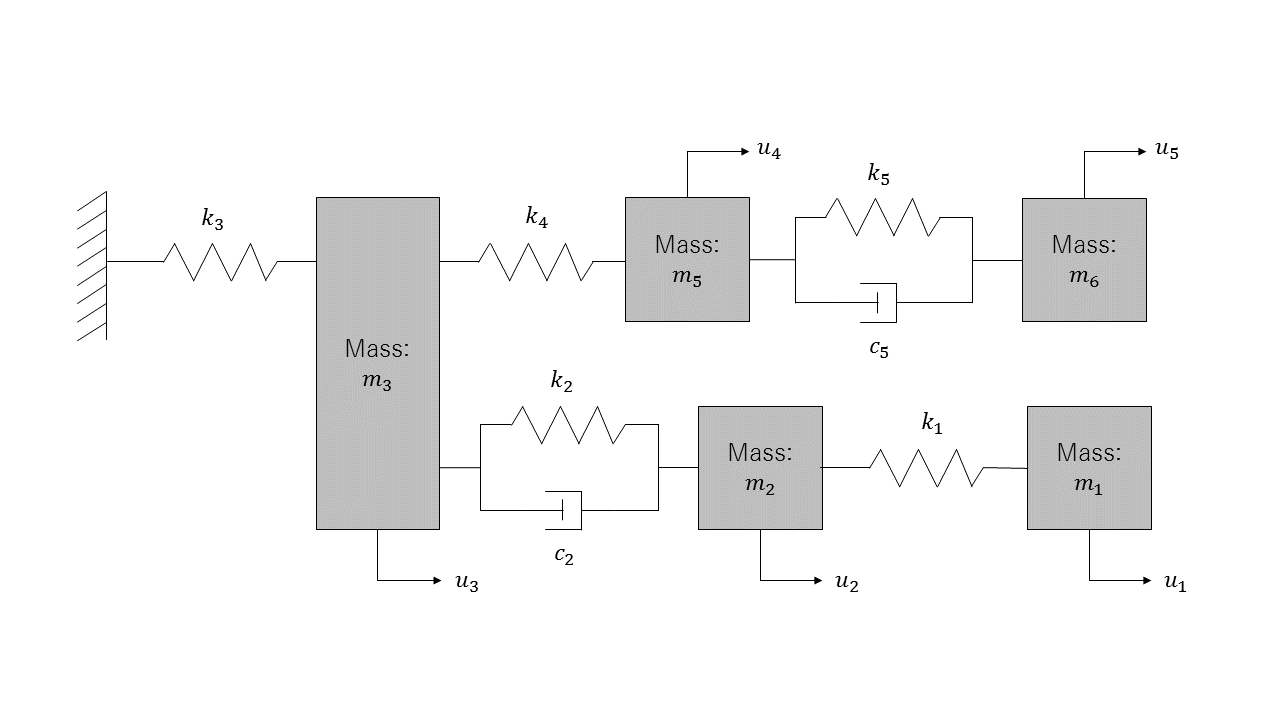
\includegraphics[width=15cm]{img/system-model.png}
    \caption{ローズピアノの簡易モデル}
    \label{fig:簡易モデル}
\end{figure}
% ![ローズ・ピアノ簡易モデル](img/system-model.png)

図はローズ・ピアノのシステムモデルである.$k$はバネ定数,$m$は質量,$u$は変位,$c$はダッシュポットである.図中上部がTonebarになり,図中下部がTineに相当する.TonebarとTineをつないでいるPoleは$m_3$に相当する.



\subsection{連立常微分方程式}

主変数 $u$ に関する連立常微分方程式は,

\begin{equation}
    M \frac{d^2 u}{dt^2} + B^T R B \frac{du}{dt} + B^T D B_u = f    
\end{equation}

である.$M$は質量マトリクス,$D$はバネマトリクス,$R$は減衰マトリクス,$B$は係数行列である.

図\ref{fig:簡易モデル}を運動方程式は,

\begin{eqnarray}
    \begin{matrix}
        m_1 \ddot{u_1} &+&  & & k_1 (u_1 - u_2) &=& 0 \\ 
        m_2 \ddot{u_2} &+& c_2(\dot{u_2} - \dot{u_1}) &+& k_2 (u_2 - u_3) + k_1 (u_2 - u_1) &=& 0 \\ 
        m_3 \ddot{u_3} &+& c_2(\dot{u_3} - \dot{u_2}) &+& k_2 (u_3 - u_2) + k_3 u_3 &=& 0 \\ 
        m_4 \ddot{u_4} &+& c_5(\dot{u_4} - \dot{u_5}) &+& k_5 (u_4 - u_5) + k_4 (u_4 - u_3) &=& 0 \\ 
        m_5 \ddot{u_5} &+& c_5(\dot{u_5} - \dot{u_4}) &+& k_5 (u_5 - u_4) &=& 0
    \end{matrix}        
\end{eqnarray}

である.運動方程式より状態方程式は,

\begin{eqnarray}
    M = 
    \left(\begin{matrix}
        m_1 & 0   & 0   & 0   & 0   & 0   \\
        0   & m_2 & 0   & 0   & 0   & 0   \\
        0   & 0   & m_3 & 0   & 0   & 0   \\
        0   & 0   & 0   & m_4 & 0   & 0   \\
        0   & 0   & 0   & 0   & m_5 & 0   \\
        0   & 0   & 0   & 0   & 0   & m_6
    \end{matrix}\right)
\end{eqnarray}

\begin{eqnarray}
    D =
    \left(\begin{matrix}
        k_1 & 0   & 0   & 0   & 0   & 0   \\
        0   & k_2 & 0   & 0   & 0   & 0   \\
        0   & 0   & k_3 & 0   & 0   & 0   \\
        0   & 0   & 0   & k_4 & 0   & 0   \\
        0   & 0   & 0   & 0   & k_5 & 0   \\
        0   & 0   & 0   & 0   & 0   & k_6
    \end{matrix}\right)
\end{eqnarray}

\begin{eqnarray}
    R = 
    \left(\begin{matrix}
        0   & 0   & 0   & 0   & 0   & 0   \\
        0   & c_2 & 0   & 0   & 0   & 0   \\
        0   & 0   & 0   & 0   & 0   & 0   \\
        0   & 0   & 0   & 0   & 0   & 0   \\
        0   & 0   & 0   & 0   & c_5 & 0   \\
        0   & 0   & 0   & 0   & 0   & c_6
    \end{matrix}\right)
\end{eqnarray}

ただし,$u_6$,$m_6$,$k_6$,$c_6$は完全固定なので$0$である.